%start preamble
\documentclass[paper=a4,fontsize=11pt]{scrartcl}%kind of doc, font size, paper size

\usepackage{fontspec}
\defaultfontfeatures{Ligatures=TeX}
%\setsansfont{Liberation Sans}
\usepackage{polyglossia}	
\setdefaultlanguage[spelling=new, babelshorthands=true]{german}
\usepackage{csquotes}
		
\usepackage{amsmath}%get math done
\usepackage{amsthm}%get theorems and proofs done
\usepackage{graphicx}%get pictures & graphics done
\graphicspath{{pictures/}}%folder to stash all kind of pictures etc
\usepackage{hyperref}%for links to web
\usepackage{amssymb}%symbolics for math
\usepackage{amsfonts}%extra fonts
\usepackage []{natbib}%citation style
\usepackage{caption}%captions under everything
\usepackage{listings}
\usepackage[titletoc]{appendix}
\numberwithin{equation}{section} 
\usepackage[printonlyused,withpage]{acronym}%how to handle acronyms
\usepackage{float}%for garphics and how to let them floating around in the doc
\usepackage{cclicenses}%license!
\usepackage{xcolor}%nicer colors, here used for links
\usepackage{wrapfig}%making graphics floated by text and not done by minipage
\usepackage{dsfont}
\usepackage{stmaryrd}
\usepackage{geometry}
\usepackage{fancyhdr}
\usepackage{menukeys}
\usepackage{enumitem}



%settings colors for links
\hypersetup{
    colorlinks,
    linkcolor={blue!50!black},
    citecolor={blue},
    urlcolor={blue!80!black}
}

\definecolor{pblue}{rgb}{0.13,0.13,1}
\definecolor{pgreen}{rgb}{0,0.5,0}
\definecolor{pred}{rgb}{0.9,0,0}
\definecolor{pgrey}{rgb}{0.46,0.45,0.48}

\pagestyle{fancy}
\lhead{Netzwerke und verteilte Systeme\\
 Übung\\ Wintersemester 2021/22}
\rhead{FB-4\\Informatik in Kultur und Gesundheit\\ HTW-Berlin}
\lfoot{Virtualisierung mit VirtualBox}
\cfoot{}
\fancyfoot[R]{\thepage}
\renewcommand{\headrulewidth}{0.4pt}
%\renewcommand{\footrulewidth}{0.4pt}

\lstdefinestyle{Bash}{
  language=bash,
  showstringspaces=false,
  basicstyle=\small\sffamily,
  numbers=left,
  numberstyle=\tiny,
  numbersep=5pt,
  frame=trlb,
  columns=fullflexible,
  backgroundcolor=\color{gray!20},
  linewidth=0.9\linewidth,
  %xleftmargin=0.5\linewidth
  upquote=true,
  columns=fullflexible,
  literate={*}{{\char42}}1
         {-}{{\char45}}1
}

\newenvironment{solution}
	{
		\color{blue}
		\textbf{Lösung:}
	}{}


%%here begins the actual document%%
\newcommand{\horrule}[1]{\rule{\linewidth}{#1}} % Create horizontal rule command with 1 argument of height


\DeclareMathOperator{\id}{id}

\title{	
\normalfont \normalsize 
\textsc{Übungsblatt 01 -- Shell Grundlagen}
}
\begin{document}
\begin{center}
\Large{\textbf{Übungsblatt 1 -- Shell Grundlagen}}
\end{center}
Diese Übung soll sie zunächst mit dem Umgang unixoider Betriebssysteme vertraut machen, sodass der Einstieg etwas leichter fällt. Im speziellen ist hier der Umgang mit der Kommandozeile gemeint, da Server-Systeme i.A. keine grafische Schnittstelle anbieten.\\
Die Erfahrung zeigt, dass einige Studierende zunächst überfordert sind. Keine Sorge: Sie sind nicht allein.\\
Generell hilft es am Ball zu bleiben und sich kontinuierlich mit den Aufgaben zu beschäftigen -- das heißt auch: selber recherchieren, Literatur lesen, sich Unklarheiten bewusst machen und entsprechende Fragen stellen.

\begin{center}\Large{\textbf{Aufgabe A -- Shell Basics}}\end{center}\vskip0.25in
%\setlist[enumerate, 1]{itemsep=\baselineskip}
\begin{enumerate}
\item Navigation:\\
Ziel dieser Aufgabe ist die grundlegende Navigation in der Shell zu verstehen.
\begin{enumerate}[label=(\alph*)]
		\item Starten sie die VM! Sie können sich als Nutzer \emph{student} mit dem Passwort \emph{student} anmelden. (Ja, das Passwort ist beim eintippen nicht zu sehen!)
		\begin{figure}[h]
		\centering
		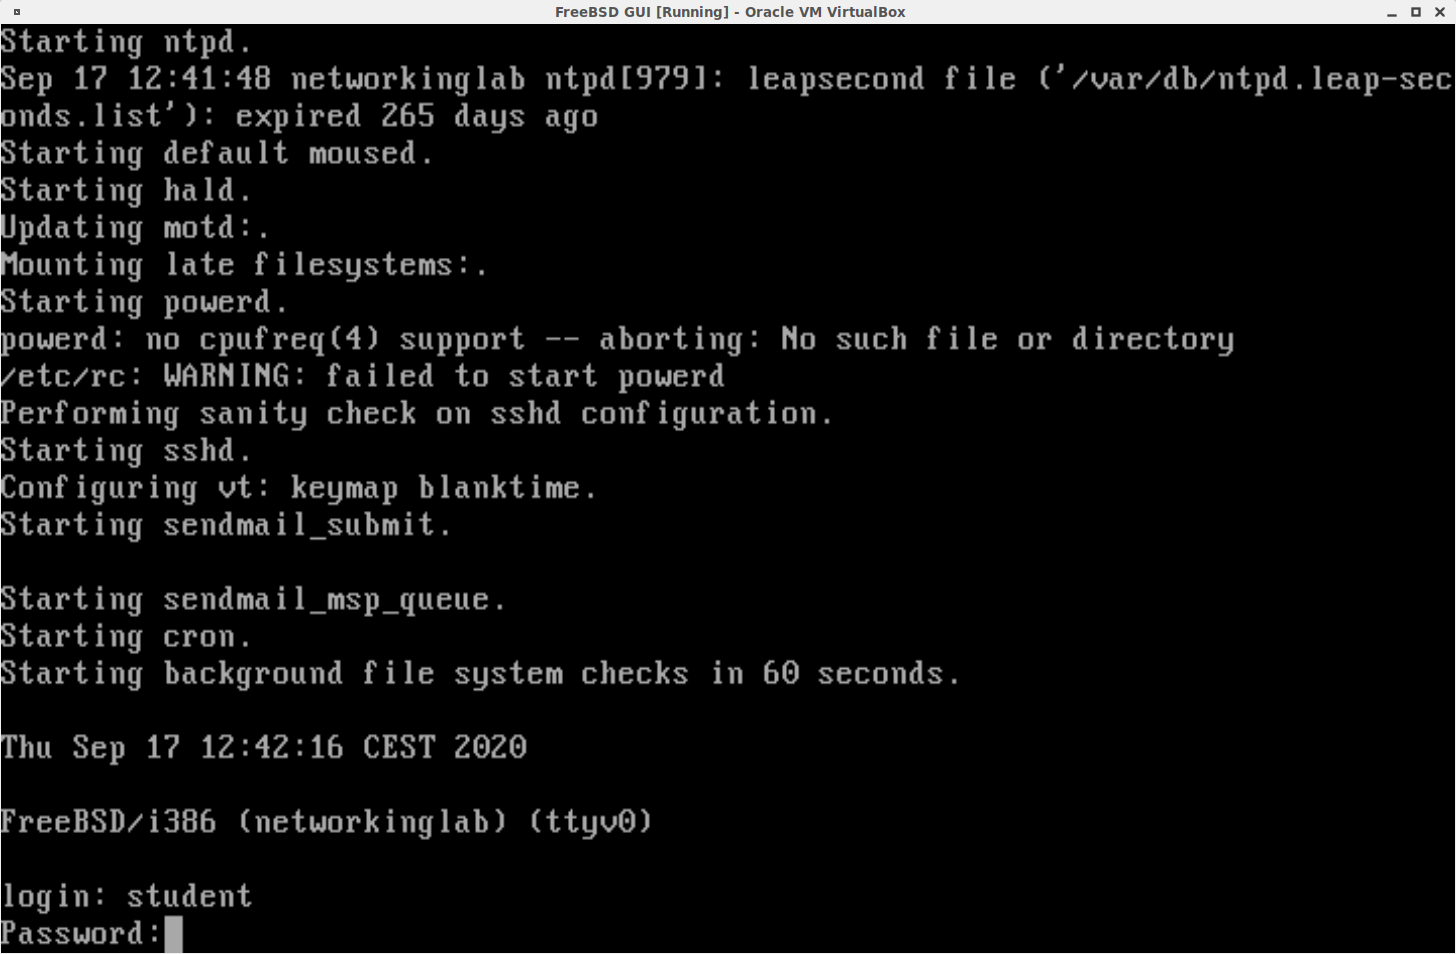
\includegraphics[scale=0.3]{freebsd_login}
		\end{figure}
		\item Mit dem Befehl \emph{startx} können sie die grafische Oberfläche starten -- müssen es aber nicht. Sie sind im Betriebssystem angemeldet und können alle Aufgabe lösen.\\
		Falls sie unter der GUI arbeiten: Starten sie die Kommandozeile (Shell)! Entweder via Tastenkombination \keys{\ctrl + \Alt + t} (STRG + ALT + T) oder über das Menü bzw. das Icon im Panel.\\
		Lassen sie sich anschließend Ihr aktuelles Verzeichnis auf der Kommandozeile ausgeben! Dies ist standardmäßig ihr Heimatverzeichnis \footnote{Auch \enquote{home directory}: $\sim$ oder ausgeschrieben \path{/home/student/} auf der VM bzw. \path{/home/s0xxxxxx} auf den Laborrechnern}.
		\item Lassen sie sich den Inhalt des Verzeichnisses mithilfe des Kommandos \emph{ls} ausgeben.
		
		\begin{solution}
		\begin{lstlisting}[style=Bash, language=Bash]
ls
		\end{lstlisting}
		\end{solution}
		\item Navigieren sie via \emph{cd} in den Ordner \path{/var}
		\begin{solution}
		\begin{lstlisting}[style=Bash, language=Bash]
cd /var
		\end{lstlisting}
		\end{solution}
		\item Springen sie von diesen Ordner in den übergeordneten Ordner (\emph{/} -- root).
		
		\begin{solution}
		\begin{lstlisting}[style=Bash, language=Bash]
cd ..
		\end{lstlisting}
		\end{solution}
		\item Navigieren sie in Ihr Heimatverzeichnis (Dies sollte durch genau ein Kommando erfolgen!)
		
		\begin{solution}
		\begin{lstlisting}[style=Bash, language=Bash]
cd 
#oder
cd ~
		\end{lstlisting}
		\end{solution}
		\item Recherchieren sie kurz den Unterschied zwischen relativen und absoluten Pfaden in Unix-Dateisystemen. Sie können folgende Quelle hierfür nutzen: \url{https://de.wikipedia.org/wiki/Pfadname}\\
		\begin{solution}
		Absolute Pfade beinhalten den Kompletten Baum des Dateisystems startend beim Wurzelelement \emph{/}. Relative Pfade sind ein Teilbaum, dessen Wurzel das aktuelle Verzeichnis ist. Der Rest des Baums ist dennoch erreichbar, nur das Wurzelelement ist im Graphen "verschoben".
		\end{solution}
		\item Lassen sie sich mit dem Befehl \emph{history} die letzten Befehle Anzeigen, die im Terminal ausgeführt wurden. 
		\begin{solution}
		\begin{lstlisting}[style=Bash, language=Bash]
history
		\end{lstlisting}
		\end{solution}
		\item Benutzen sie die Pfeiltasten \keys{\arrowkeyup} und \keys{\arrowkeydown}, um die letzten Befehle auf die Kommandozeile zu bringen. Mithilfe der Pfeiltasten können sie durch die Historie der bereits genutzten Befehle navigieren, wobei \keys{\arrowkeyup} in Richtung älterer Befehle und \keys{\arrowkeydown} Richtung neuerer springt.
		\item Mit der Tastenkombination \keys{\ctrl +r} öffnen Sie die interaktive Suche der History anstoßen. Unter Ihrem Command-Prompt erscheint folgendes:\\
		\begin{lstlisting}[style=Bash, language=Bash]
bck-i-search: _
		\end{lstlisting}
		Mithilfe dieser Suche können sie nach bereits benutzten Befehlen suchen. Wenn sie beispielsweise \emph{cd} eingeben sehen Sie den zuletzt genutzten Befehl der den Token \emph{cd} enthält. Durch wiederholtes Drücken der Tastenkombination \keys{\ctrl +r} durchsuchen Sie die History Richtung älterer Befehle die das angegebene Schlüsselwort enthalten.\\
		\textbf{Kommandos:} \textcolor{blue}{\emph{cd}, \emph{pwd}, \emph{history}}
	\end{enumerate}
	\item Grundlegende Kommandos:\\
  Um den grundlegenden Umgang mit der Shell kennenzulernen fertigen Sie sich ein eigenes kleines Shell-Tutorial an.\\
  \textbf{Hinweis:} Um lästige Tipparbeit zu vermeiden, bieten viele Shells eine Autovervollständigung an. Mit der \keys{\tab}-Taste (Tabulatortaste) kann diese genutzt werden -- sie müssen lediglich die ersten Buchstaben tippen und können durch (mehrmaliges) drücken der Tabulatortaste den begonnenen Befehl vervollständigen. Wenn es mehrere Alternativen der Vervollständigung gibt, kann zwischen diesen gesprungen werden.\\
  Schauen sie in die Aufgabe B, wenn bestimmte Kommandos (noch) nicht wie gewünscht arbeiten! Ein Blick in die Hilfe löst dies in vielen Fällen.
  	\begin{enumerate}[label=(\alph*)]
  		\item Erzeugen sie das Verzeichnis \path{shell_tutorial} und wechseln sie in das erzeugte Verzeichnis. Erzeugen sie darin eine leere Datei mit dem Dateinamen \textit{shell\_tutorial.md}.\footnote{.md steht für Markdown, welches ein Format für Textdateien ist, ähnlich wie .txt oder .doc-Dateien.} (\textbf{Der Satzpunkt gehört nicht zum Dateinamen!})\\
        \textbf{Achtung:} Verwenden sie zum Anlegen der Datei keinen Editor, sondern (einen) Kommandozeilenbefehl(e).\\
        \textbf{Kommandos:} \textcolor{blue}{\emph{touch}, \emph{mkdir}, \emph{cd}}
        
        \begin{solution}
        \begin{lstlisting}[style=Bash, language=Bash]
mdkir shell_tutorial
cd shell_tutorial
touch shell_tutorial.md
		\end{lstlisting}
		\end{solution}
		\item Überprüfen sie die Dateigröße der Datei \textit{shell\_tutorial.md}.\\
		\textbf{Kommandos:} \textcolor{blue}{\emph{ls}, \emph{stat}, \emph{du}}
		
		\begin{solution}
        \begin{lstlisting}[style=Bash, language=Bash]
du -h shell_tutorial.md # Groesse in Bytes auf der Platte, 4KB ist die Standardblockgroesse, auch wenn die Datei kleiner ist.
ls -la shell_tutorial.md #in Bytes vor dem Datum
stat shell_tutorial.md # wie bei du
		\end{lstlisting}
		\end{solution}
		\item Fügen sie mithilfe der Umleitung der Standardausgabe die Zeilen "Shell Tutorial", sowie eine (neue) Zeile mit dem aktuellen Datum in die Datei \path{shell_tutorial.md} ein.\\
		\textbf{Kommandos:} \textcolor{blue}{\emph{echo}, \emph{date}, $>>$, bzw. \emph{>}}
		\begin{itemize}
			\item \small Verwenden sie für das Einfügen des Textes keinen Editor, sondern einen Befehl und eine Weiterleitung (Umleitung der Standardausgabe).
		\end{itemize}
		
		\begin{solution}
        \begin{lstlisting}[style=Bash, language=Bash]
#einfache Variante
echo "shell tutorial" > shell_tutorial.md
date >> shell_tutorial.md
#schoener
(echo "shell tutorial"; date) > shell_tutorial.md
#oder
(printf "shell tutorial\n"; date) > shell_tutorial.md
		\end{lstlisting}
		\end{solution}
		\item Geben sie die erste Zeile der Datei \path{shell_tutorial.md} auf der Kommandozeile aus.\\
		\textbf{Kommandos:} \textcolor{blue}{\emph{head}, \emph{tail}, \emph{more}, \emph{less}}
		
		\begin{solution}
        \begin{lstlisting}[style=Bash, language=Bash]
head -n 1 shell_tutorial.md
		\end{lstlisting}
		\end{solution}
		\item Öffnen sie Ihr Cheat-Sheet mithilfe das Programms \emph{vim}, \emph{emacs} oder via \emph{retext}. Notieren sie sich alle Befehle, sowie deren Bedeutung, sodass sie eine erste Anlaufstelle für die nächsten Übungen haben. Dieses Dokument (Sie können auch mehrere anlegen) sollten sie fortan als Notizzettel für die Laboraufgaben nutzen!
		\item Navigieren sie in Ihr Heimatverzeichnis. Legen sie folgenden Ordner, sowie Unterordner mithilfe des \emph{mkdir}-Kommandos an: \path{exercise_notes/tutorials}. (Satzpunkt gehört wieder nicht zum Dateinamen!)
		
		\begin{solution}
        \begin{lstlisting}[style=Bash, language=Bash]
cd
mkdir -p exercise_notes/tutorials
		\end{lstlisting}
		\end{solution}
		\item Kopieren sie die Datei bzw. den Ordner \emph{shell\_tutorial} in das eben angelegte Verzeichnis.\\
		\textbf{Kommandos:} \textcolor{blue}{\emph{cp} }
		
		\begin{solution}
        \begin{lstlisting}[style=Bash, language=Bash]
#kopiere nur Datei
cp shell_tutorial/shell_tutorial.md exercise_notes/tutorials
#Ordner
cp -r shell_tutrial exercise_notes/tutorials
		\end{lstlisting}
		\end{solution}
        \item Kopieren sie die Datei(en) inklusive des Ordners \path{exercises/tutorials/shell_tutorial.md} in das Verzeichnis \path{/tmp}.\\
        \textbf{Hinweise:} Schauen sie in die Manpage von \emph{cp} um herauszufinden, wie Ordner kopiert werden können.\\
        \textbf{Kommandos:} \textcolor{blue}{\emph{man cp}}
        
		\begin{solution}
        \begin{lstlisting}[style=Bash, language=Bash]
cp -r shell_tutorial /tmp
		\end{lstlisting}
		\end{solution}
  	\end{enumerate}
  	\footnote{.md steht für Markdown, welches ein Format für Textdateien ist, ähnlich wie .pdf oder .doc-Dateien.}
\newpage  
         \item Benutzer- \& Systeminfos:
    		\begin{enumerate} [label=(\alph*)]
          \item Lassen sie sich den Nutzernamen und die Gruppenzugehörigkeit auf dem Terminal des Rechners ausgeben.\\
          \textbf{Kommandos:} \textcolor{blue}{\emph{id}, \emph{groups}, \emph{whoami}}
          
		\begin{solution}
        \begin{lstlisting}[style=Bash, language=Bash]
# id numerisch via user IDs oder group IDs + symbolisch
id
#groups nur die Namen der Gruppen, ohne uid oder gid
groups
# nur Nutzername
whoami
		\end{lstlisting}
		\end{solution}
          \item Lassen sie sich den Namen ihrer VM ausgeben.\\
          \textbf{Kommandos:} \textcolor{blue}{\emph{hostname}}

		\begin{solution}
        \begin{lstlisting}[style=Bash, language=Bash]
hostname
		\end{lstlisting}
		\end{solution}
          \item Legen sie einen Ordner \emph{.nfo} an. Schreiben Sie die Ausgaben Ihres Nutzernamens, Gruppenzugehörigkeit sowie den Namen des genutzten Rechners in die Datei \emph{info.nfo} in den Ordner \emph{.nfo}.
          
		\begin{solution}
        \begin{lstlisting}[style=Bash, language=Bash]
mkdir .nfo
(id; hostname) > .nfo/info.nfo
		\end{lstlisting}
		\end{solution}
          \item Nutzen sie \emph{ls} und prüfen sie, ob sie den Ordner wiederfinden können! Finden sie heraus, wie sie mithilfe des \emph{ls} Kommandos trotzdem diesen versteckten Ordner (Hidden-Folder) finden können.
          
		\begin{solution}
        \begin{lstlisting}[style=Bash, language=Bash]
# Dateien die mit . beginnen (Punktdateien/Dotfiles) sind "versteckt"
ls -la
		\end{lstlisting}
		\end{solution}
          \item Löschen sie erst die \emph{info.nfo}-Datei. Anschließend den Ordner \emph{.nfo}\\
          \textbf{Kommandos:} \textcolor{blue}{\emph{rm}}
          
		\begin{solution}
        \begin{lstlisting}[style=Bash, language=Bash]
rm .nfo/info.nfo
rm -r .nfo
		\end{lstlisting}
		\end{solution}
          \item Wie findens sie heraus, welche Benutzer noch auf dem ihrer VM eingeloggt sind und wie lange diese angemeldet sind.\\
          \textbf{Kommandos:} \textcolor{blue}{\emph{who}, \emph{last}, \emph{lastlog}}
          		\begin{solution}
        \begin{lstlisting}[style=Bash, language=Bash]
#aktuell angemeldet
who
#wer war zuletzt auf dem System
last
#lastlog letzter login aller vorhanden Nutzer
lastlog
		\end{lstlisting}
		\end{solution}
          \item Bringen sie das genutzte Betriebssystem, sowie dessen Kernel in Erfahrung.\\
          
		\begin{solution}
        \begin{lstlisting}[style=Bash, language=Bash]
#uname nur OS
uname
# OS + Kernel etc
uname -a
freebsd-version
		\end{lstlisting}
		\end{solution}
          \textbf{Kommandos:} \textcolor{blue}{\emph{freebsd-version}, \emph{uname}}
          \item Viele Unix-Systeme haben eine Quota -- eine Beschränkung des Speicherverbrauchs, ist diese auf der VM vorhanden? Falls ja, wie sieht diese aus?\\
          \textbf{Kommandos:} \textcolor{blue}{\emph{quota}}
          
		\begin{solution}
        Kein Quota-System vorhanden
		\end{solution}
          \item Wie sie der verfügbare Plattenplatz aus?\\
          \textbf{Kommandos:} \textcolor{blue}{\emph{df -h}}
          
		\begin{solution}
        \begin{lstlisting}[style=Bash, language=Bash]
# ohne -h in Bytes
df -h
		\end{lstlisting}
		\end{solution}
        \end{enumerate}
        \item Anlegen eines eigenen Nutzers:
        \begin{enumerate}
        		\item Legen sie einen eigenen Nutzer an. Dieser soll fortan für die Übungen als Admin-Account benutzt werden.
        		\item Gehen sie die Fragen Schrittweise durch. (s. Abb.).
        		\begin{itemize}
        			\item Geben sie einen Nutzername ein (freie Wahl)
        			\item Lassen sie \emph{UID}, \emph{Login-Group} unverändert (einfach Enter/return).
        			\item Bei Group-Invite soll ihr neuer Account der Gruppe \emph{wheel} angehören! Das ist notwendig, um mit erhöhten Rechten arbeiten zu können.
        			\item Die Login-Class kann unverändert bleiben.
        			\item Wählen sie eine Shell (ich empfehle ZSH oder BASH)
        			\item Gehen sie die Passwortabfrage durch. Wählen sie, wie ihr Passwort aussehen soll (leer, zufällig, oder nutzergewählt). Wenn sie selbst das Passwort wählen, legen sie dies fest (Eingabe nicht sichtbar) und wiederholen sie dies anschließend.
        			\item Wenn alle Eingaben stimmen, fragt sie das System, ob ihre Eingaben korrekt sind und trägt diese anschließend ein.
       			\item In der unteren Abb. sehen sie, wie dies beispielhaft aussehen könnte.
       			\begin{figure}[h]
       			\centering
       			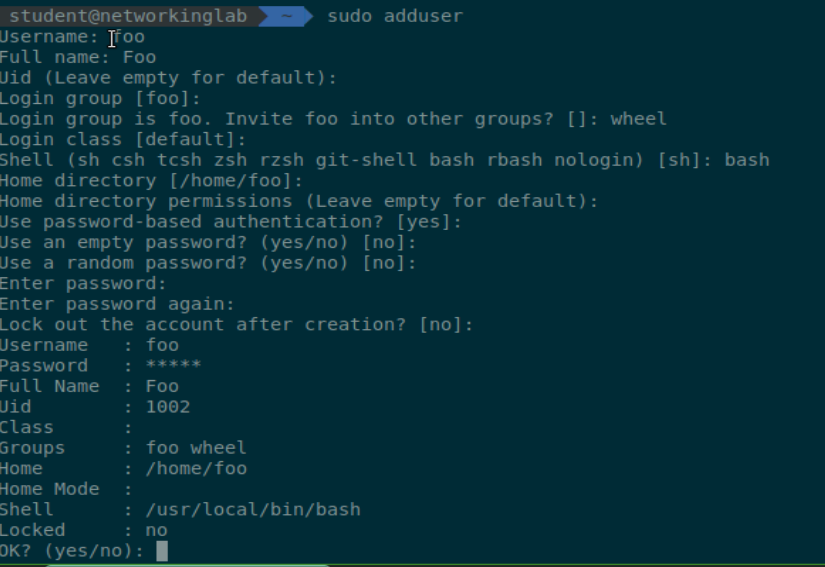
\includegraphics[scale=0.4]{add_user}
       			\end{figure}
        		\end{itemize}
        \end{enumerate}
        \item Sudo -- Recherchieren sie, wie und was der Befehl \emph{sudo} leisten kann.\\
        Eine Anlaufstelle wäre: \url{https://www.freebsd.org/doc/de_DE.ISO8859-1/books/handbook/security-sudo.html}
        
		\begin{solution}
		\emph{sudo} für "Super User Do" (oder "Substitute User Do"). Nutzer ohne root-Privilegien, die das System administrieren sollen (teilweise) Zugriffe auf Ressourcen bekommen, die erhöhte Privilegien benötigen. Daher können Nutzer oder ganze Gruppen von Nutzer vollen oder Teilzugriff bekommen. Hierfür gibt es die \path{/etc/sudoers} via \emph{sudoedit}. root-Nutzer dürfen im System alles, d.h. wenn mit root-Rechten gearbeitet wird, sollte man aufpassen.\\
		Alternative zu sudo: \emph{doas} aus dem \emph{openBSD} Betriebssystem. Ähnlich wie sudo, nur besser durchdacht und deutlich besser programmiert.
		\end{solution}
\end{enumerate}

\begin{center}\Large{\textbf{Aufgabe B -- Manpages \& Hilfe}}\end{center}\vskip0.25in
Unix bietet von Hause aus einige Anlaufstellen an, mit deren Hilfe sie die Handhabung von der Tools (Kommandozeilenbefehle etc.) recherchieren können.
\begin{enumerate}
	\item Suchen sie sich einen Befehl aus den sie heute bereits benutzt haben. Mithilfe der Parameter \emph{--help}, \emph{-help} oder \emph{-h} erhalten Sie eine kurze Übersicht über den Befehl.
    \item Rufen sie die \emph{manpage} für einen beliebigen Befehl ein: \\
    		\emph{man HIERBEFEHLKEINFUEGEN}\\
		 Nutzen sie die Pfeiltasten, die Bild hoch/runter (\keys{pageup \arrowkeyup}/ \keys{pageup \arrowkeydown}) oder Leertaste (\keys{\Space}) zum lesen. Schließen erfolgt mit \keys{q}. Mit \emph{/} könne sie innerhalb der Manpage suchen.
\end{enumerate}
Die Manpages finden sie als Website auch im Internet. \footnote{\url{https://linux.die.net/man/}}

\begin{center}\Large{\textbf{Aufgabe C -- User \& Rechte}}\end{center}\vskip0.25in
%\setlist[enumerate, 1]{itemsep=\baselineskip}
\begin{enumerate}
\item Diskrete Zugangskontrolle (DAC) -- Nutzer \& Gruppen
	\begin{enumerate}[label=(\alph*)]
        \item Recherchieren sie die Bedeutung der Spalten 1 -- 7 der Ausgabe des Kommandos \emph{ls -la} in ihrem Heimatverzeichnis.
        
        \begin{solution}
         \begin{enumerate}
        		\item Dateityp
        		\item Rechte User-Gruppe-Others in symbolischer Schreibweise
        		\item Anzahl der Links
        		\item Name des Dateieigentümers
        		\item Name der Gruppenzugehörigkeit
        		\item Dateigröße (in Bytes)
        		\item Datum der letzten Änderung
        		\item Datei- oder Ordnername
        \end{enumerate}
        \end{solution}
        \item Finden sie die Datei bzw. das Programm \textit{reboot}, die den Neustart des Systems veranlassen kann. Lassen Sie sich die Rechte der Datei \textit{reboot} ausgeben!
        \textbf{Kommandos:} \textcolor{blue}{\emph{whereis}, \emph{find}}
        
        \begin{solution}
        \begin{lstlisting}[style=Bash, language=Bash]
#mit whereis
whereis reboot
#alternativ
find / -type f -name "reboot" 2>& 1 | grep -v "Permission denied"
		\end{lstlisting}
		\end{solution}
        \item Um was für einen Dateitypen handelt es sich hierbei? Was ist reboot für eine Datei -- recherchieren Sie gegebenenfalls kurz.
        
        \begin{solution}
        \begin{lstlisting}[style=Bash, language=Bash]
# gibt den Dateitypen wieder, ELF32 Binary
file /sbin/reboot
ls -la /sbin/reboot
		\end{lstlisting}
		\end{solution}
        \item Wer ist der Eigentümer, wie sehen die Berechtigungen für Nutzer, Gruppe und Andere in symbolischer, oktaler und binärer Schreibweise aus?
        
        \begin{solution}
        \begin{lstlisting}[style=Bash, language=Bash]
ls -la /sbin/reboot # Eingentuemer root Gruppe: wheel
		\end{lstlisting}
		Berechtigungen: Nutzer: r-x, Gruppe: r-x, Others: r-x $to$ r-xr-xr-x; oktal; 555; binär: 101 101 101
		\end{solution}
        \item Schreiben sie die Ergebnisse der vorigen Aufgabe in die Datei \textit{reboot\-\_permission.txt}.
        \item Nennen sie Möglichkeiten den Inhalt der Datei \textit{reboot\-\_permission.txt} anzeigen lassen. Welche Rechte besitzt diese Datei?
        
        \begin{solution}
        Rechte: Nutzer der Datei angelegt hat Lese- und Schreibrechte, alle anderen nur Leserechte. 
        \begin{lstlisting}[style=Bash, language=Bash]
cat reboot_permission.txt
head rp.txt
less rp.txt
more rp.txt
		\end{lstlisting}
		\end{solution}
        \item Wie würde das Kommando lauten um die Rechte der Datei \textit{reboot\-\_permission.txt} so zu ändern, sodass der Nutzer lesen und schreiben kann, Nutzer der gleichen Gruppe nur lesen und alle anderen keinen Zugriff haben. (Jeweils oktal und symbolisch.) 
        
        \begin{solution}
        \begin{lstlisting}[style=Bash, language=Bash]
chmod u=rw,g=r,o=- reboot_permission.txt
chmod 540 reboot_permission.txt
		\end{lstlisting}
		\end{solution}
        \item Können sie den Rechner mit dem Kommando \textit{reboot} neu starten? Falls nicht, warum?
        
        \begin{solution}
       	Dem Rechtesystem nach ja: denn das Execute-Bit ist für \emph{others} gesetzt. Das Betriebssystem erlaubt dies dennoch nicht. Da im allgemeinen nicht jeder Nutzer das OS neu starten können soll.
        \end{solution}
        \item Führen sie einen Reboot des Systems durch -- Achtung speichern sie alle offenen Dateien, sodass sie keine ungespeicherten Daten verlieren!
  \end{enumerate}
  \item Was ist nach dem Neustart aus dem Ordner der Aufgabe \texttt{A Shell Basic -- 2h)} geworden?
  
  \begin{solution}
  Dateien im \path{/tmp} sind temporäre Dateien, d.h. nach einem Neustart sind diese weg.
  \end{solution}
\end{enumerate}
\begin{center}\Large{\textbf{vi/vim}}\end{center}\vskip0.25in
\begin{enumerate}
	\item Der Standardeditor unter Unix ist \emph{vi}, dieser ist auf jedem System vorhanden. Bearbeiten Sie folgendes Tutorial:\\
	\url{http://www.openvim.com/}\\
	Ein Cheat-Sheet kann unter:\\
	\url{https://www.fprintf.net/vimCheatSheet.html}\\
	bezogen werden, sodass die Nutzung etwas leichter fällt.\\
	Sie müssen kein vi-Guru werden, jedoch sollten Sie wissen, wie Dateien geöffnet, geschlossen, gespeichert werden, sowie wie im vi/vim navigiert wird und wie Sie den vi verlassen können. Notieren Sie sich in Ihrem Cheat-Sheet wie Sie vorgegangen sind!\\
	Die Navigation in den Manpages entspricht der des vims.
	\item Nutzen sie den \emph{vi(m)}-Editor, um den Hostnamen der virtuellen Maschine zu ändern. Sie können einen beliebigen Namen wählen, es empfiehlt sich einen Namen zu wählen, der die Funktionalität widerspiegelt.
\end{enumerate}

\begin{center}\Large{\textbf{Reboot \& Poweroff}}\end{center}\vskip0.25in
\begin{enumerate}
	\item Sie können das System mit dem Befehlt \emph{sudo reboot} neu starten.
	\item Mithilfe des Befehls \emph{poweroff} können sie das System herunterfahren.
\end{enumerate}

Weiter geht es mit dem zweiten Übungsblatt: Netzwerkinfrastruktur 1!

\end{document}